\documentclass{article}
\usepackage{iclr2026_conference,times}
\usepackage{hyperref}
\usepackage{url}
\usepackage{amsmath,amssymb}
\usepackage{booktabs,multirow,array}
\usepackage{microtype}
\usepackage{graphicx}
\usepackage{float}

\newcommand{\fix}{\marginpar{FIX}}
\newcommand{\new}{\marginpar{NEW}}

\iclrfinalcopy

\title{AgentKit: A Hybrid Planning Agent for Dynamic Emergency\\
Response Allocation with Clone-Based Lookahead\\
and Conditional LLM Arbitration}

\author{Akhil Gogineni, Nicolas Yepes, Akshat Bhat, \& Trusha Talati \\
Department of Computer Science\\
University of Illinois Urbana-Champaign\\
Champaign, IL 61820, USA \\
\texttt{\{vg23,nyepes2,akshatb5,ttalati2\}@illinois.edu}
}

\begin{document}
\maketitle

\begin{abstract}
We present \textbf{AgentKit}, a hybrid planning agent for dynamic emergency
resource allocation evaluated on \textbf{RescueBench}, a 20-scenario
four-tier benchmark on a 16-node city graph with heterogeneous fleets,
multi-capability incidents, and timed infrastructure failures.
AgentKit combines deterministic feasibility enforcement with
\emph{clone-based rollout}: before each dispatch it deep-copies the world,
simulates top candidates forward, projects benchmark scores, and commits to
the best lookahead outcome; an LLM arbitrator resolves ties within an 8\%
margin using Memory Log context.
We introduce \emph{Cap-PWRS}, a capability-coverage metric with a linear late
penalty that captures partial multi-vehicle progress beyond binary PWRS.
Against a deterministic greedy baseline and a zero-shot LLM baseline,
AgentKit achieves mean PWRS \textbf{0.615} vs.\ 0.592 and 0.566, with zero
constraint violations across all 20 scenarios.
The gain concentrates on Tier~3 (ethical prioritization under vehicle
scarcity): \textbf{0.807} vs.\ 0.719 (deterministic, $+8.8$ pp) and 0.615
(zero-shot, $+19.2$ pp).
Tier~4 scores are identical across all methods, confirming that replanning
cannot recover from mid-mission infrastructure failures.
\end{abstract}

%% ─────────────────────────────────────────────────────────────────
\section{Introduction}
\label{sec:intro}

Emergency resource allocation requires both semantic prioritization and
mathematical precision.
LLMs reason fluently about competing urgencies but hallucinate routes, dispatch
uncapable vehicles, and lose track of committed resources across multi-step
interactions.
Deterministic heuristics avoid these failures but cannot perform the
non-local look-ahead needed to resolve scarcity tradeoffs.

\textbf{AgentKit} closes this gap: all routing, feasibility checking, and
execution are deterministic; the planning layer generates a pre-validated
candidate shortlist; clone-based rollout projects each candidate's downstream
PWRS before commitment; and an LLM is consulted \emph{only} when rollout
cannot clearly separate the top candidates.
We evaluate on \textbf{RescueBench}, 20 scenarios across four difficulty tiers
with entirely deterministic grading.

\paragraph{Related work.}
\citet{yao2023react} showed ReAct-style tool use grounds LLM decisions;
we restrict the LLM to a pre-validated shortlist, eliminating open-ended
constraint violations~\citep{schick2023toolformer,shinn2023reflexion}.
Traditional dispatch uses greedy heuristics and integer
programming~\citep{zhang2017ems,liu2019multi}; LLM-based planners have not
been systematically evaluated here prior to this work.
Our clone-based rollout is a deterministic analogue of MCTS
rollouts~\citep{browne2012mcts}, providing noise-free projected scores for
candidate comparison.
Tier~2 instantiates cooperative multi-vehicle
dispatch~\citep{stone2000,khamis2015} not previously studied under LLM
agents.

\paragraph{Contributions.}
(1)~\textbf{RescueBench}: 20-scenario benchmark, four tiers, deterministic
grading.
(2)~\textbf{AgentKit}: hybrid agent with clone-based rollout and conditional
LLM arbitration, zero constraint violations.
(3)~\textbf{Cap-PWRS}: capability-coverage metric with linear late penalty.
(4)~Three-method comparative evaluation showing $+8.8$ pp PWRS on Tier~3
with no regression elsewhere.

%% ─────────────────────────────────────────────────────────────────
\section{Benchmark and Metrics}
\label{sec:benchmark}

\paragraph{RescueBench.}
20 JSON scenarios share a 16-node city graph (24 directed edges with
per-edge \texttt{allowed\_vehicle\_types} restrictions) and a fleet of four
vehicle types (ambulance, fire truck, police unit, supply truck).
Incidents carry \texttt{required\_capabilities} sets; resolution requires
every capability to be covered by a dispatched vehicle arriving before the
deadline.
A Gemini-powered pipeline generated scenarios from a hand-authored base
graph, computing tight-but-feasible deadlines via Dijkstra and injecting
timed dynamic triggers (bridge collapses, road floods, fire spread).

\textbf{Tier~1} (Basic Triage): single-capability incidents, ample fleet.
\textbf{Tier~2} (Multi-Capability): incidents require coordinated
multi-vehicle coverage; edge restrictions and fuel constraints active.
\textbf{Tier~3} (Scarcity): fleet capacity exactly covers the major incident
\emph{or} the minor incidents, not both; the agent must solve the
severity-weighted tradeoff.
\textbf{Tier~4} (Dynamic Replanning): hidden triggers fire mid-mission,
collapsing roads after vehicles are already committed.

\paragraph{Metrics.}
$\text{PWRS} = \bigl(\sum_i s_i \cdot \mathbf{1}[\text{resolved}_i \wedge
t_i^* \leq d_i]\bigr) \big/ \sum_i s_i$
awards severity-weighted credit only for on-time resolutions.
Cap-PWRS awards partial credit for capability coverage with a linear
late penalty:
\begin{equation}
  \text{Cap-PWRS} = \frac{\displaystyle\sum_i s_i \cdot
    \frac{|C_i^{\text{cov}} \cap C_i^{\text{req}}|}{|C_i^{\text{req}}|}
    \cdot \max\!\left(0,\,1 - \tfrac{\max(0,\,t_i^*-d_i)}{d_i}\right)}
  {\displaystyle\sum_i s_i}.
  \label{eq:cappwrs}
\end{equation}
We additionally report resolution rate, deadline adherence, violation count,
and step efficiency (resolved incidents per dispatch step).

%% ─────────────────────────────────────────────────────────────────
\section{Agent Design}
\label{sec:agent}

\subsection{Shared Infrastructure}

All methods share the same deterministic simulator.
\textbf{WorldState} maintains the city graph (with per-edge closure state),
concurrent vehicle missions, incident coverage tracking, hospital admission
state, and a dynamic-triggers schedule; time advances via an event-driven
model that jumps to the next vehicle-release or trigger-fire.
\textbf{WorldTool} exposes six API functions for querying and acting.
\textbf{ValidatorTool} deterministically gates every proposed dispatch:
vehicle availability, non-zero capability contribution, fuel, hospital
capacity, and vehicle-type-aware Dijkstra routing must all pass before a
dispatch executes.

\subsection{AgentKit}
\label{sec:agentkit}

AgentKit runs an \textbf{observe~$\to$ plan~$\to$ act~$\to$
wait\,/\,replan} loop (Figure~\ref{fig:architecture}).

\begin{figure}[t]
  \centering
  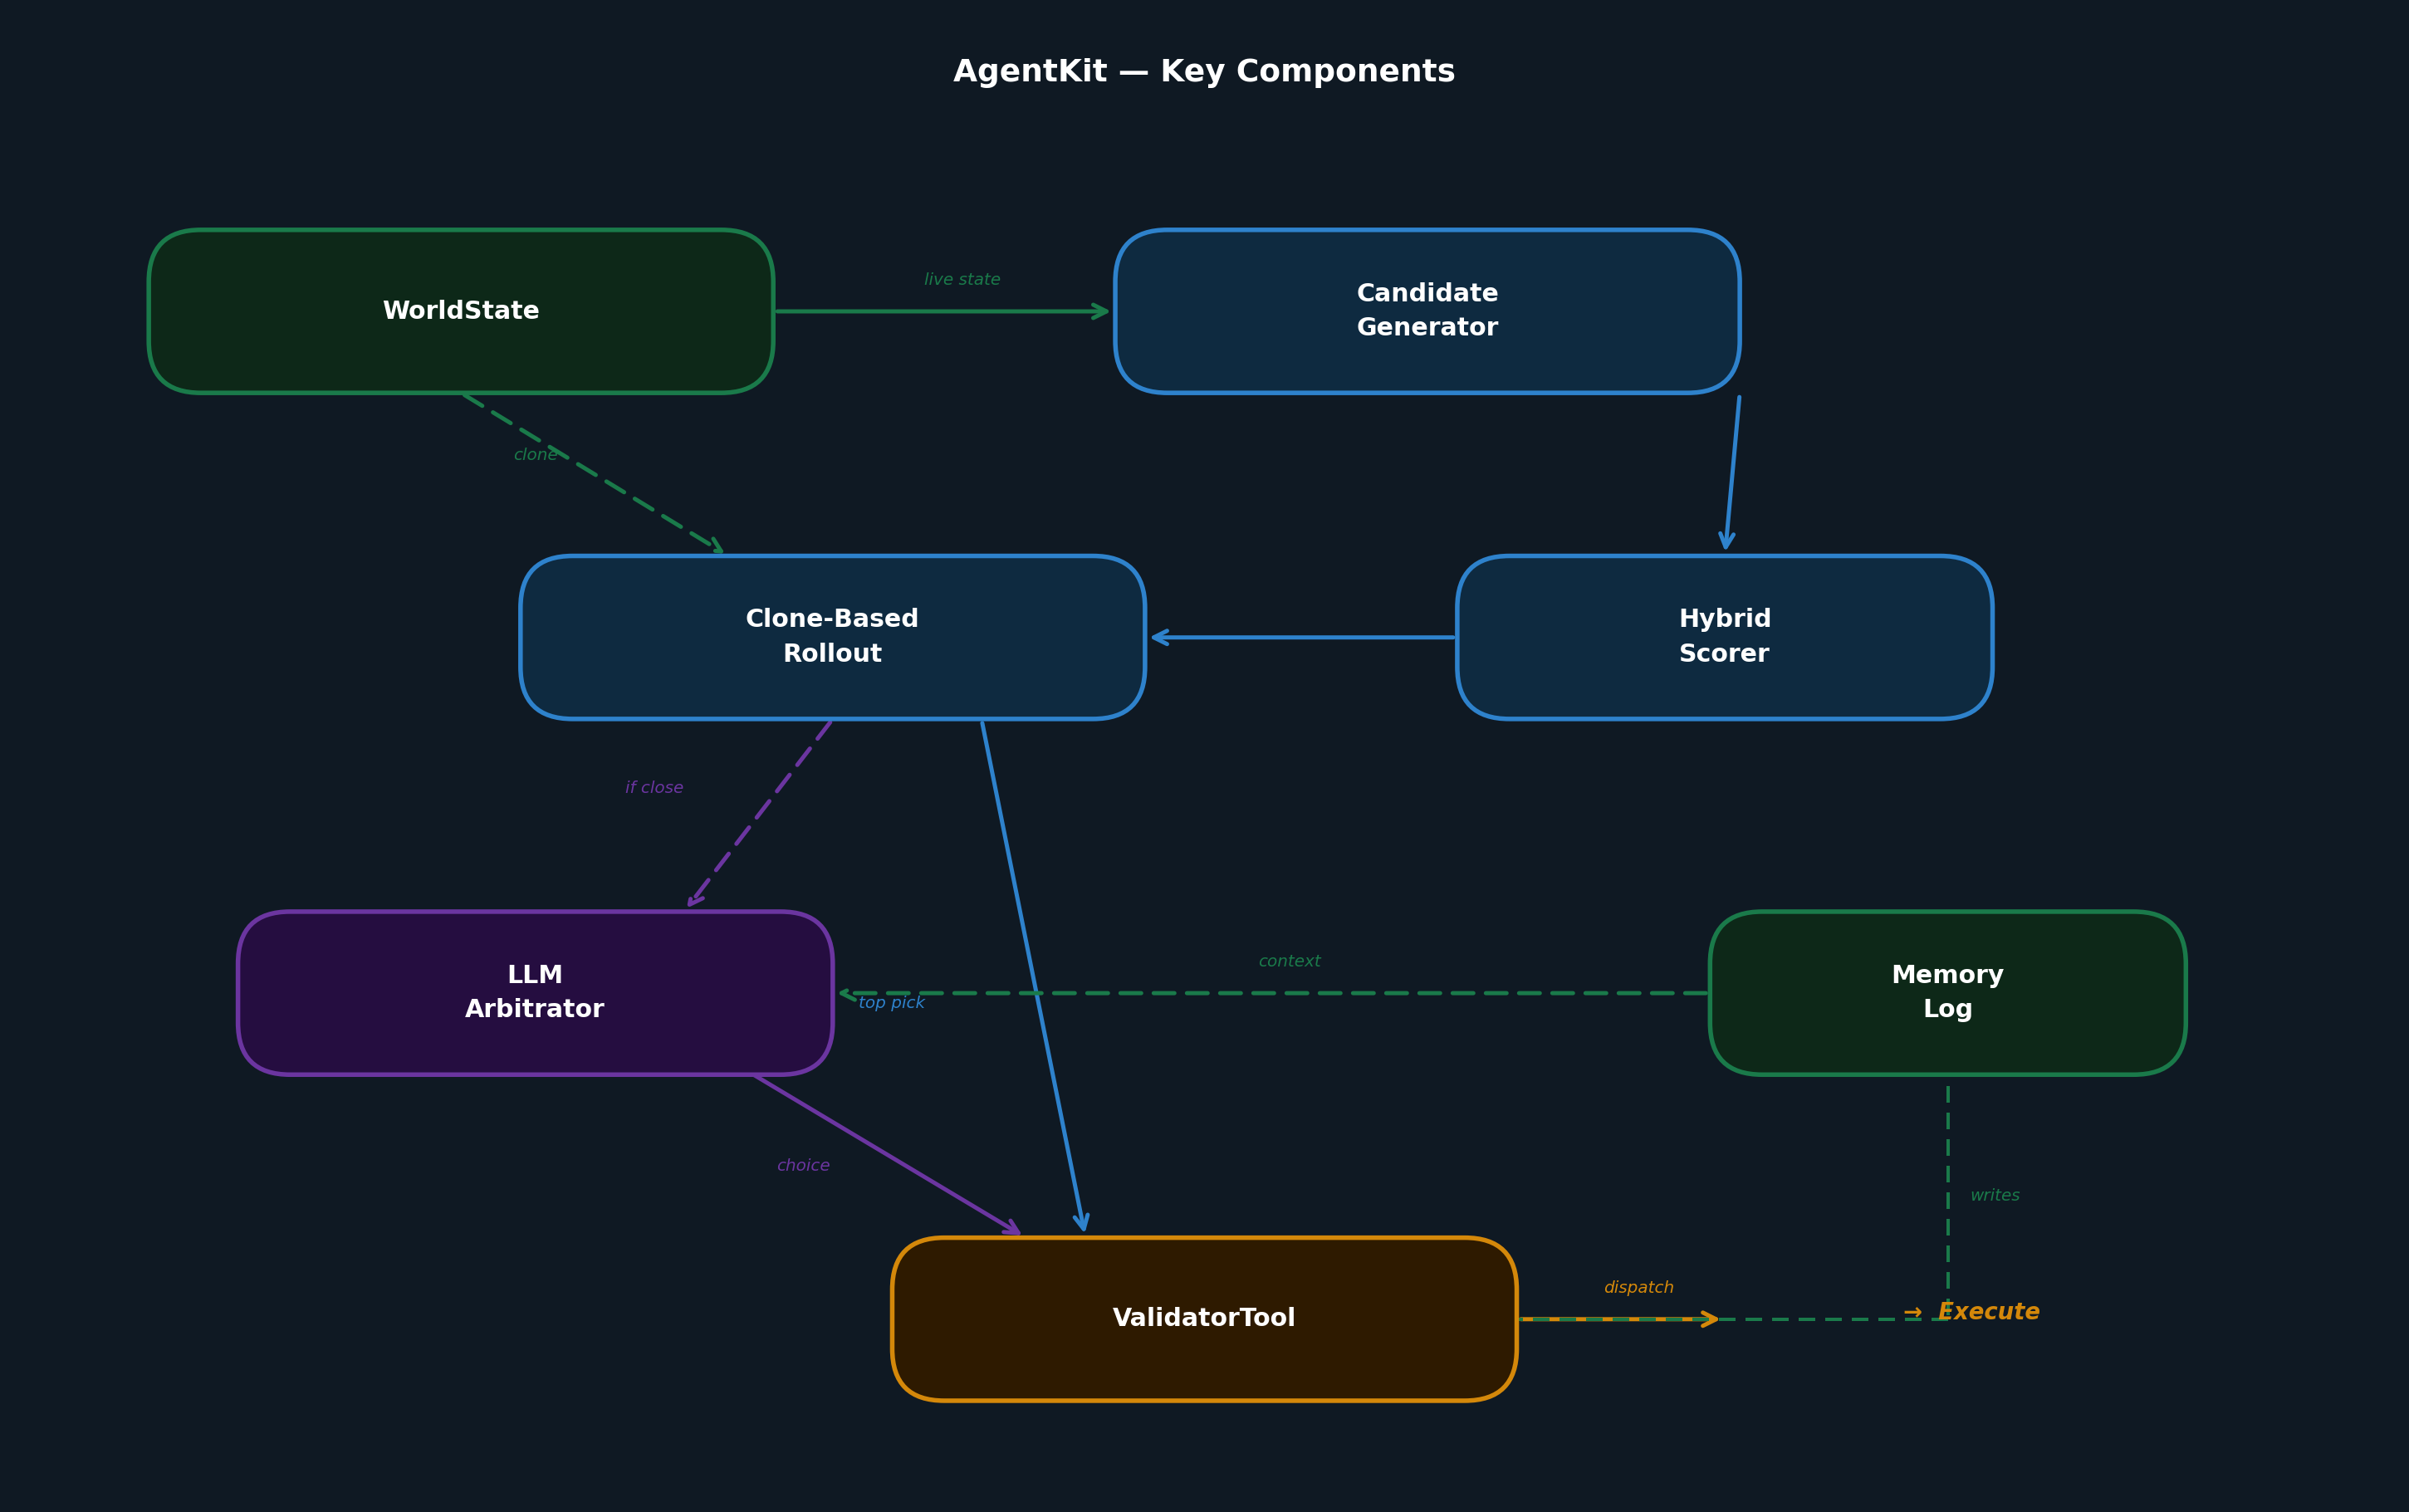
\includegraphics[width=0.80\textwidth]{agentkit_architecture.png}
  \caption{AgentKit pipeline.  Candidates are pre-validated, scored, and
    projected via clone-based rollout before commitment.  The LLM
    Arbitrator is invoked only when the rollout gap is $\leq$8\%.
    ValidatorTool gates every dispatch path.}
  \label{fig:architecture}
\end{figure}

\textbf{Observe} polls world state and proactively fires all pending
dynamic triggers, ensuring infrastructure failures are detected every
cycle.
\textbf{Plan} ranks open incidents by $(-\text{severity}, +\text{deadline})$;
the LLM is consulted only when the top two share identical severity
\emph{and} deadline.
\textbf{Candidate Generation} evaluates every idle vehicle against every
open incident: a vehicle enters the pool only if it (a)~covers at least
one uncovered required capability, (b)~passes ValidatorTool
pre-validation, and (c)~has a finite Dijkstra path.
Each candidate receives a heuristic pre-score
$\propto \text{severity} \times \text{deadline\_pressure} \times
\text{remaining\_work}$, plus a scarcity bonus
$1/\max(1,\text{provider\_count})$ and a \emph{future-option cost}
penalizing vehicles that are the sole feasible responder for a different
open incident.
The top-12 proceed to rollout.

\textbf{Clone-Based Rollout} evaluates each shortlisted candidate by
deep-copying WorldState, executing the candidate dispatch, running the
deterministic greedy policy for up to 4 additional steps inside the clone,
and calling \texttt{compute\_metrics} to obtain projected PWRS and
Cap-PWRS.
The candidate with the highest projected PWRS is the rollout winner.

\textbf{LLM Arbitration:} if the rollout winner leads the runner-up by
more than 8\% on projected PWRS, it proceeds directly to ValidatorTool.
Otherwise, the top-5 rollout candidates plus the last 5 Memory Log entries
(blocked states, prior LLM choices, dynamic alerts) are sent to the LLM,
which selects one candidate by ID.
In both cases the selection passes through ValidatorTool before execution.

\textbf{Wait\,/\,Replan:} after each dispatch, \texttt{advance\_to\_next\_event}
jumps to the nearest vehicle-release or trigger event.
If alerts fire, \texttt{replan()} flushes and rebuilds the plan queue from
fresh world state.

\subsection{Baselines}

\textbf{Deterministic:} same observe/plan/act/wait loop; candidate
selection is direct greedy --- first available vehicle contributing to
the highest-priority incident.  No LLM calls.

\textbf{Zero-Shot LLM:} a single prompt with the full scenario description
is sent to \texttt{claude-sonnet-4-5}; the model returns a JSON dispatch
list executed in order.  Violations are logged and skipped.

%% ─────────────────────────────────────────────────────────────────
\section{Results}
\label{sec:results}

\paragraph{Setup.}
Deterministic and AgentKit run 3 times per scenario (mean reported);
Zero-Shot runs once.  All LLM calls use \texttt{claude-sonnet-4-5}.

\begin{table}[t]
\centering
\caption{Per-tier results. \textbf{Bold}: best per column per tier.
  AgentKit achieves zero violations on all tiers.
  Step efficiency (Eff.) is N/A for Zero-Shot (no iterative tool steps).}
\label{tab:main}
\footnotesize
\renewcommand{\arraystretch}{1.05}
\begin{tabular}{llccccccc}
\toprule
\textbf{Method} & \textbf{Tier} &
  \textbf{PWRS} & \textbf{Cap-PWRS} &
  \textbf{Res.} & \textbf{DL~Adh.} &
  \textbf{Viol.} & \textbf{Step~Eff.} \\
\midrule
Zero-Shot       & 1 & \textbf{0.745} & \textbf{0.931} & \textbf{1.000} & \textbf{0.767} & 0.0 & N/A \\
Zero-Shot       & 2 & \textbf{0.400} & \textbf{0.903} & \textbf{1.000} & \textbf{0.400} & 0.2 & N/A \\
Zero-Shot       & 3 & 0.615          & 0.615          & 0.433          & 0.433          & 0.0 & N/A \\
Zero-Shot       & 4 & \textbf{0.506} & \textbf{0.797} & \textbf{0.800} & \textbf{0.500} & 0.0 & N/A \\
\midrule
Deterministic   & 1 & \textbf{0.745} & \textbf{0.931} & \textbf{1.000} & \textbf{0.767} & \textbf{0.0} & \textbf{1.000} \\
Deterministic   & 2 & \textbf{0.400} & \textbf{0.903} & \textbf{1.000} & \textbf{0.400} & \textbf{0.0} & 0.567 \\
Deterministic   & 3 & 0.719          & 0.820          & 0.900          & 0.567          & \textbf{0.0} & 0.800 \\
Deterministic   & 4 & \textbf{0.506} & \textbf{0.797} & \textbf{0.800} & \textbf{0.500} & \textbf{0.0} & \textbf{0.500} \\
\midrule
AgentKit (Ours) & 1 & \textbf{0.745} & \textbf{0.931} & \textbf{1.000} & \textbf{0.767} & \textbf{0.0} & \textbf{1.000} \\
AgentKit (Ours) & 2 & \textbf{0.400} & \textbf{0.903} & \textbf{1.000} & \textbf{0.400} & \textbf{0.0} & 0.567 \\
AgentKit (Ours) & 3 & \textbf{0.807} & \textbf{0.864} & \textbf{0.900} & \textbf{0.700} & \textbf{0.0} & 0.800 \\
AgentKit (Ours) & 4 & \textbf{0.506} & \textbf{0.797} & \textbf{0.800} & \textbf{0.500} & \textbf{0.0} & \textbf{0.500} \\
\bottomrule
\end{tabular}
\end{table}

\begin{table}[t]
\centering
\caption{Mean across all four tiers.}
\label{tab:summary}
\small
\renewcommand{\arraystretch}{1.05}
\begin{tabular}{lccccc}
\toprule
\textbf{Method} & \textbf{Mean PWRS} & \textbf{Mean Cap-PWRS} &
  \textbf{Mean Res.} & \textbf{Mean DL Adh.} & \textbf{Mean Viol.} \\
\midrule
Zero-Shot LLM   & 0.566 & 0.812 & 0.808 & 0.525 & 0.050 \\
Deterministic   & 0.592 & 0.863 & 0.925 & 0.559 & \textbf{0.000} \\
AgentKit (Ours) & \textbf{0.615} & \textbf{0.874} & \textbf{0.925} & \textbf{0.592} & \textbf{0.000} \\
\bottomrule
\end{tabular}
\end{table}

\paragraph{Tiers~1, 2, and~4.}
All three methods score identically on PWRS and Cap-PWRS on these tiers,
confirming that AgentKit never regresses.
Zero-Shot incurs 0.2 violations per Tier~2 run (e.g., MED\_03 dispatched
to INC\_CRASH\_001 where its capabilities were already fully covered) ---
a failure pre-validated candidate generation prevents by requiring
non-empty contribution before shortlisting.
Tier~4 results are identical across all methods because the failures are
structural: dynamic triggers collapse roads after vehicles are already
mid-mission and cannot be recalled, making replanning irrelevant to the
affected dispatches.

\paragraph{Tier~3: look-ahead advantage.}
AgentKit scores PWRS~\textbf{0.807} vs.\ 0.719 (Deterministic) and 0.615
(Zero-Shot).
The gain is entirely attributable to clone-based rollout identifying
non-obvious vehicle-reuse sequences.
In scenario~13, one police unit must serve both a riot (severity 0.9,
ETA 11.7 min) and a traffic incident (severity 0.7, ETA 6.7 min).
Greedy ordering dispatches to the riot first; the vehicle returns too
late for the traffic deadline (PWRS~0.850).
Rollout projects that serving the traffic call first (6.7 min round trip)
frees the vehicle in time to still resolve the riot (PWRS~1.000), and
AgentKit commits to that sequence.
Deadline adherence on Tier~3 rises from 0.567 (Deterministic) to
\textbf{0.700} (AgentKit), reflecting consistently better sequencing
across all five scenarios.

%% ─────────────────────────────────────────────────────────────────
\section{Discussion and Conclusion}
\label{sec:conclusion}

\paragraph{Clone-based rollout is the source of improvement.}
Without rollout, AgentKit degenerates to the Deterministic baseline
(identical PWRS on Tiers~1, 2, and~4).
Rollout depth~5 is sufficient to project vehicle-reuse sequences ---
dispatch A, wait for return, dispatch A again --- that lie at the heart
of Tier~3 tradeoffs.
Because rollout produces clean numerical scores, the LLM arbitration
path triggers only when candidates are genuinely indistinguishable,
bounding LLM call budget without sacrificing the zero-violation guarantee.

\paragraph{LLM in a constrained role.}
Zero-Shot violations arise because an unconstrained LLM lacks an explicit
model of per-incident uncovered-capability state.
By restricting LLM selection to a pre-validated shortlist, AgentKit
eliminates this failure class entirely while retaining LLM judgment for
contextual disambiguation at the margin.

\paragraph{Limitations.}
Dispatched vehicles cannot be recalled mid-mission, the direct cause of
every Tier~4 failure and a constraint shared by all methods.
Results cover 20 scenarios on a fixed 16-node graph; generalization to
larger graphs is unvalidated.
All LLM experiments use a single model (\texttt{claude-sonnet-4-5}).

\paragraph{Conclusion.}
AgentKit achieves zero constraint violations and a mean PWRS of 0.615
($+8.8$ pp over deterministic on Tier~3, $+19.2$ pp over zero-shot)
by combining deterministic candidate pre-validation, clone-based rollout
look-ahead, and bounded LLM arbitration restricted to a pre-validated
shortlist --- a pattern we believe generalizes well beyond emergency
dispatch to any constrained sequential decision problem.

%% ─────────────────────────────────────────────────────────────────
\begin{thebibliography}{99}
\small

\bibitem[Browne et al.(2012)]{browne2012mcts}
Browne, C.~B., et al.
A survey of Monte Carlo tree search methods.
\textit{IEEE Trans.\ Comp.\ Intel.\ AI Games}, 4(1):1--43, 2012.

\bibitem[Chevalier-Boisvert et al.(2019)]{chevalier2019babyai}
Chevalier-Boisvert, M., et al.
BabyAI: A platform to study the sample efficiency of grounded language learning.
\textit{ICLR}, 2019.

\bibitem[Chen et al.(2022)]{chen2022code}
Chen, M., et al.
Evaluating large language models trained on code.
\textit{arXiv:2107.03374}, 2022.

\bibitem[Gogineni et al.(2026)]{group2bench2026}
Gogineni, A., Yepes, N., Bhat, A., and Talati, T.
RescueBench: A tiered benchmark for emergency response allocation agents.
Technical report, UIUC CS~498, 2026.

\bibitem[Khamis et al.(2015)]{khamis2015}
Khamis, A., Hussein, A., and Elmogy, A.
Multi-robot task allocation: A review.
\textit{Cooperative Robots and Sensor Networks}, pp.\ 31--51. Springer, 2015.

\bibitem[Liu et al.(2019)]{liu2019multi}
Liu, Y., et al.
Multi-objective vehicle routing optimization for emergency logistics.
\textit{Transportation Research Part C}, 107:321--340, 2019.

\bibitem[Schick et al.(2023)]{schick2023toolformer}
Schick, T., et al.
Toolformer: Language models can teach themselves to use tools.
\textit{NeurIPS}, 2023.

\bibitem[Shinn et al.(2023)]{shinn2023reflexion}
Shinn, N., et al.
Reflexion: Language agents with verbal reinforcement learning.
\textit{NeurIPS}, 2023.

\bibitem[Shridhar et al.(2021)]{shridhar2021alfworld}
Shridhar, M., et al.
ALFWorld: Aligning text and embodied environments for interactive learning.
\textit{ICLR}, 2021.

\bibitem[Stone \& Veloso(2000)]{stone2000}
Stone, P. and Veloso, M.
Multiagent systems: A survey from a machine learning perspective.
\textit{Autonomous Robots}, 8(3):345--383, 2000.

\bibitem[Yao et al.(2023)]{yao2023react}
Yao, S., et al.
ReAct: Synergizing reasoning and acting in language models.
\textit{ICLR}, 2023.

\bibitem[Zhang \& Li(2017)]{zhang2017ems}
Zhang, Z.-H. and Li, K.
A novel probabilistic formulation for locating and sizing EMS stations.
\textit{Annals of Operations Research}, 229(1):813--835, 2017.

\end{thebibliography}

\end{document}
